\documentclass[12pt,letterpaper]{report}
\usepackage[utf8]{inputenc}
\usepackage[T1]{fontenc}
\usepackage[english]{babel}
\usepackage{amsmath}
\usepackage{amsfonts}
\usepackage{amssymb}
\usepackage{graphicx}

\title{Charge Pump Derivation}
\author{Ryan J. Billing}

\begin{document}
	\maketitle
	\begin{figure}
		\centering
		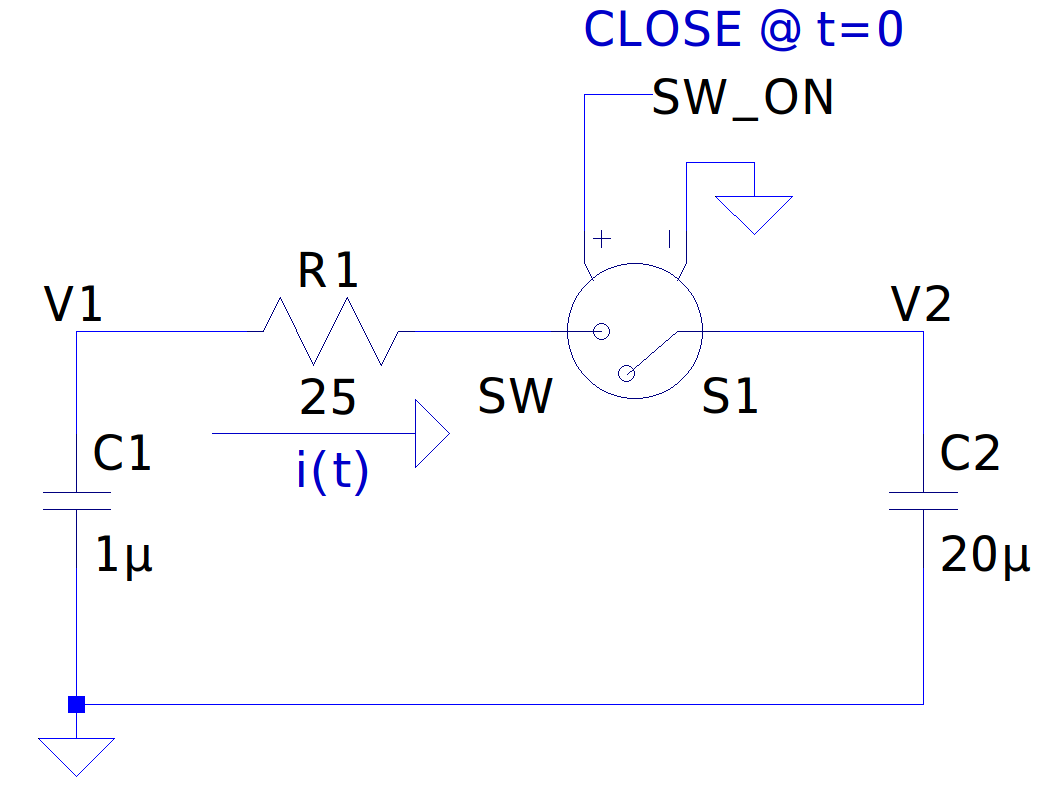
\includegraphics[width=0.7\linewidth]{img/charge_pump_discharge_cycle}
		\caption{Charge Pump discharge cycle operation}
		\label{fig:chargepumpdischargecycle}
	\end{figure}
	
	\section{Initial observations}
	Figure \ref{fig:chargepumpdischargecycle} depicts part of a charge pump circuit during the discharging cycle.  $C_1$ is the flying capacitor that was charged to a voltage of $V_1$.  At time $t=0$ the switch $S_1$ will close and $C_1$ will begin to discharge into $C_2$.
	
	The goal of this exercise is to determine how much energy is dissipated in R1 and determine the final voltage after the circuit has stabilized.  A closed-form solution for $i(t)$ is determined, it can be used to quantify how much charge is transferred from $C_1$ to $C_2$ in this scenario.   The final voltages, $V_1$ and $V_2$, can be determined from the integral of $i_t$ by subtracting this charge from $C_1$ or adding it to $C_2$.  In the final settled state it is apparent that $V_1 = V_2$.
	
	\section{Useful relationships}
	This section presents a set of fundamental relationships that may be used to determine the function for $i(t)$.
	
	\begin{align}
		i(t) &= -C_1 \frac{dV_1}{dt} \label{c1deriv} \\
		i(t) &= C_2 \frac{dV_2}{dt} \label{c2deriv} \\
		i(t) &= \frac{V_1(t) - V_2(t)}{R_1} \label{itV}
	\end{align}

	\section{Derivation of i(t)}
	First find $V_1$ and $V_2$ from equations (\ref{c1deriv}) and (\ref{c2deriv}).  
	
	\begin{align}
		V_1(t) &= -\frac{1}{C_1} \int i(t) dt \text{ (Negative sign because current is going out of $C_1$)} \nonumber \\
		V_2(t) &= \frac{1}{C_2} \int i(t) dt
	\end{align}
	
	Plug these into (\ref{itV}) and then solve the resulting differential equation for $i(t)$.
	
	\begin{align}
		i(t) &= -\frac{1}{R_1} \bigg( \frac{1}{C_1} \int i(t) dt -\frac{1}{C_2} \int i(t) dt\bigg)
	\end{align}

	Next differentiate and collect like terms.
	
	\begin{align}
		\frac{di(t)}{dt} &= - \frac{\frac{1}{C_1} + \frac{1}{C_2}}{R_1} i(t) \nonumber \\
		R_1 \frac{C_1 C_2}{C_1 + C_2} \bigg ( \frac{1}{i(t)}\bigg) \frac{di(t)}{dt} &= -1
	\end{align}

	Integrating both sides.
	
	\begin{align}
		R_1 \frac{C_1 C_2}{C_1 + C_2} \int \frac{1}{i(t)} dt  &= \int -1 dt \\
		R_1 \frac{C_1 C_2}{C_1 + C_2} \bigg( ln\big(i(t)\big) + C\bigg) &= -t \\
		ln\big(i(t)\big) + C &= -t  \frac{C_1 + C_2}{R_1 C_1 C_2}
	\end{align}

	Exponentiate to solve for $i(t)$,
	
	\begin{align}
		e^{ln\big(i(t)\big)} e^{C} &= e^{-t \frac{C_1 + C_2}{ R_1C_1 C_2}} \nonumber \\
		i(t) &= e^{-C} e^{-t  \frac{C_1 + C_2}{ R_1C_1 C_2}} \label{it_general}
	\end{align}

	Finally the integration constant can be determined by considering the initial conditions,
	
	\begin{align}
		i(0) &= \frac{V_1(0) - V_2(0)}{R_1}
	\end{align}

	The expression (\ref{it_general}) is solved for the known initial conditions at $t=0$ to determine the yet unknown constant of integration.  In this case the constant $C$ itself is a "don't care" quantity as we really want to know $e^{-C}$ directly so the entire expression may be expressed in terns of initial voltages and the resistor value.
	
	\begin{align}
		\frac{V_1(0) - V_2(0)}{R_1} &=  e^{-C} e^{-0  \frac{C_1 + C_2}{R_1 C_1 C_2}} \nonumber \\
		 \frac{V_1(0) - V_2(0)}{R_1} &=  e^{-C} 1 \nonumber \\
		 e^{-C} &= \frac{V_1(0) - V_2(0)}{R_1} \label{intconst}
	\end{align}

	Plugging (\ref{intconst}) into(\ref{it_general}), a closed-form expression for the resistor current, $i(t)$, is obtained.
	
	\begin{align}
		i(t) &= \frac{V_1(0) - V_2(0)}{R_1}  e^{-t \frac{(C_1 + C_2)}{R_1 C_1 C_2}} 
	\end{align}
	
	Then to help tidy the appearance of things, let
	
	\begin{align}
		V_1(0) &= V_{i1} \\
		V_2(0) &= V_{i2} \\
		\tau &= \frac{1}{ \frac{C_1 + C_2}{R_1 C_1 C_2} } = R_1 \frac{C_1 C_2}{C_1 + C_2}
	\end{align}

	And then the final expression reveals a familiar time domain response. In fact, the circuit could be redrawn as a single capacitor and resistor network driven by a step response with amplitude $V_{i1} - V_{i2}$, and where the capacitor value is equivalent to the series combination of $C_1$ and $C_2$.
	
	\begin{align}
	i(t) &= \frac{V_{i1} - V_{i2}}{R_1}  e^{-\frac{t}{\tau}} 
	\end{align}
	

\end{document}